\documentclass[]{book}
\usepackage{lmodern}
\usepackage{amssymb,amsmath}
\usepackage{ifxetex,ifluatex}
\usepackage{fixltx2e} % provides \textsubscript
\ifnum 0\ifxetex 1\fi\ifluatex 1\fi=0 % if pdftex
  \usepackage[T1]{fontenc}
  \usepackage[utf8]{inputenc}
\else % if luatex or xelatex
  \ifxetex
    \usepackage{mathspec}
  \else
    \usepackage{fontspec}
  \fi
  \defaultfontfeatures{Ligatures=TeX,Scale=MatchLowercase}
\fi
% use upquote if available, for straight quotes in verbatim environments
\IfFileExists{upquote.sty}{\usepackage{upquote}}{}
% use microtype if available
\IfFileExists{microtype.sty}{%
\usepackage[]{microtype}
\UseMicrotypeSet[protrusion]{basicmath} % disable protrusion for tt fonts
}{}
\PassOptionsToPackage{hyphens}{url} % url is loaded by hyperref
\usepackage[unicode=true]{hyperref}
\hypersetup{
            pdftitle={Bayesian Data Analysis Workbook},
            pdfauthor={Alex Liebscher},
            pdfborder={0 0 0},
            breaklinks=true}
\urlstyle{same}  % don't use monospace font for urls
\usepackage{natbib}
\bibliographystyle{apalike}
\usepackage{color}
\usepackage{fancyvrb}
\newcommand{\VerbBar}{|}
\newcommand{\VERB}{\Verb[commandchars=\\\{\}]}
\DefineVerbatimEnvironment{Highlighting}{Verbatim}{commandchars=\\\{\}}
% Add ',fontsize=\small' for more characters per line
\usepackage{framed}
\definecolor{shadecolor}{RGB}{248,248,248}
\newenvironment{Shaded}{\begin{snugshade}}{\end{snugshade}}
\newcommand{\KeywordTok}[1]{\textcolor[rgb]{0.13,0.29,0.53}{\textbf{#1}}}
\newcommand{\DataTypeTok}[1]{\textcolor[rgb]{0.13,0.29,0.53}{#1}}
\newcommand{\DecValTok}[1]{\textcolor[rgb]{0.00,0.00,0.81}{#1}}
\newcommand{\BaseNTok}[1]{\textcolor[rgb]{0.00,0.00,0.81}{#1}}
\newcommand{\FloatTok}[1]{\textcolor[rgb]{0.00,0.00,0.81}{#1}}
\newcommand{\ConstantTok}[1]{\textcolor[rgb]{0.00,0.00,0.00}{#1}}
\newcommand{\CharTok}[1]{\textcolor[rgb]{0.31,0.60,0.02}{#1}}
\newcommand{\SpecialCharTok}[1]{\textcolor[rgb]{0.00,0.00,0.00}{#1}}
\newcommand{\StringTok}[1]{\textcolor[rgb]{0.31,0.60,0.02}{#1}}
\newcommand{\VerbatimStringTok}[1]{\textcolor[rgb]{0.31,0.60,0.02}{#1}}
\newcommand{\SpecialStringTok}[1]{\textcolor[rgb]{0.31,0.60,0.02}{#1}}
\newcommand{\ImportTok}[1]{#1}
\newcommand{\CommentTok}[1]{\textcolor[rgb]{0.56,0.35,0.01}{\textit{#1}}}
\newcommand{\DocumentationTok}[1]{\textcolor[rgb]{0.56,0.35,0.01}{\textbf{\textit{#1}}}}
\newcommand{\AnnotationTok}[1]{\textcolor[rgb]{0.56,0.35,0.01}{\textbf{\textit{#1}}}}
\newcommand{\CommentVarTok}[1]{\textcolor[rgb]{0.56,0.35,0.01}{\textbf{\textit{#1}}}}
\newcommand{\OtherTok}[1]{\textcolor[rgb]{0.56,0.35,0.01}{#1}}
\newcommand{\FunctionTok}[1]{\textcolor[rgb]{0.00,0.00,0.00}{#1}}
\newcommand{\VariableTok}[1]{\textcolor[rgb]{0.00,0.00,0.00}{#1}}
\newcommand{\ControlFlowTok}[1]{\textcolor[rgb]{0.13,0.29,0.53}{\textbf{#1}}}
\newcommand{\OperatorTok}[1]{\textcolor[rgb]{0.81,0.36,0.00}{\textbf{#1}}}
\newcommand{\BuiltInTok}[1]{#1}
\newcommand{\ExtensionTok}[1]{#1}
\newcommand{\PreprocessorTok}[1]{\textcolor[rgb]{0.56,0.35,0.01}{\textit{#1}}}
\newcommand{\AttributeTok}[1]{\textcolor[rgb]{0.77,0.63,0.00}{#1}}
\newcommand{\RegionMarkerTok}[1]{#1}
\newcommand{\InformationTok}[1]{\textcolor[rgb]{0.56,0.35,0.01}{\textbf{\textit{#1}}}}
\newcommand{\WarningTok}[1]{\textcolor[rgb]{0.56,0.35,0.01}{\textbf{\textit{#1}}}}
\newcommand{\AlertTok}[1]{\textcolor[rgb]{0.94,0.16,0.16}{#1}}
\newcommand{\ErrorTok}[1]{\textcolor[rgb]{0.64,0.00,0.00}{\textbf{#1}}}
\newcommand{\NormalTok}[1]{#1}
\usepackage{longtable,booktabs}
% Fix footnotes in tables (requires footnote package)
\IfFileExists{footnote.sty}{\usepackage{footnote}\makesavenoteenv{long table}}{}
\usepackage{graphicx,grffile}
\makeatletter
\def\maxwidth{\ifdim\Gin@nat@width>\linewidth\linewidth\else\Gin@nat@width\fi}
\def\maxheight{\ifdim\Gin@nat@height>\textheight\textheight\else\Gin@nat@height\fi}
\makeatother
% Scale images if necessary, so that they will not overflow the page
% margins by default, and it is still possible to overwrite the defaults
% using explicit options in \includegraphics[width, height, ...]{}
\setkeys{Gin}{width=\maxwidth,height=\maxheight,keepaspectratio}
\IfFileExists{parskip.sty}{%
\usepackage{parskip}
}{% else
\setlength{\parindent}{0pt}
\setlength{\parskip}{6pt plus 2pt minus 1pt}
}
\setlength{\emergencystretch}{3em}  % prevent overfull lines
\providecommand{\tightlist}{%
  \setlength{\itemsep}{0pt}\setlength{\parskip}{0pt}}
\setcounter{secnumdepth}{5}
% Redefines (sub)paragraphs to behave more like sections
\ifx\paragraph\undefined\else
\let\oldparagraph\paragraph
\renewcommand{\paragraph}[1]{\oldparagraph{#1}\mbox{}}
\fi
\ifx\subparagraph\undefined\else
\let\oldsubparagraph\subparagraph
\renewcommand{\subparagraph}[1]{\oldsubparagraph{#1}\mbox{}}
\fi

% set default figure placement to htbp
\makeatletter
\def\fps@figure{htbp}
\makeatother

\usepackage{booktabs}

\title{Bayesian Data Analysis Workbook}
\author{Alex Liebscher}
\date{2020-08-05}

\begin{document}
\maketitle

{
\setcounter{tocdepth}{1}
\tableofcontents
}
\chapter{Introduction}\label{introduction}

Contained within this notebook is an approximate following of Bayesian
Data Analysis (3rd edition) by Gelman, Carlin, Stern, Dunson, Vehtari,
and Rubin (2020).

My goal is to follow the book, with as few jumps as necessary, and copy
their work, their writing, and their code. Through this, I hope to learn
how to apply Bayesian principles to the everyday data analysis problem.

Most of the text used in this workbook is paraphrased directly from the
original without shame. Their examples are sufficient and in many cases
I would do a disservice altering their language. This workbook is simply
an exercise to practice active reading, note-taking, and implementation.
It is an opportunity to learn something about Bayesian inference from a
collection of bright scholars to whom I trust to present a thorough,
captivating read of the subject.

I anticipate this to be highly interactive, which is why I've opted to
work directly in a \texttt{bookdown} format. Hopefully, some nice plots
will be created along the way.

Some code might be compared to
\href{https://github.com/avehtari/BDA_R_demos}{Aki Vehtari's}. Vehtari
also has published their
\href{https://github.com/avehtari/BDA_course_Aalto}{own lecture notes},
which could also be a helpful resource. Luckily too, it seems like most
of the data is hosted on Gelman's site - this should come in handy.

\section{Collaboration}\label{collaboration}

I am looking for a reading group to incrementally work through the
textbook and have discussions with. If you are looking to learn about
Bayesian inference, I hope you won't be shy and we can struggle
together. Email me at \texttt{alexliebscher0@gmail.com} and just say
you're interested, I'll figure out the rest.

Moreover, feel free to clone this repo for a quick start.

\chapter{Probability and Inference}\label{intro}

Bayesian data analysis may be broken down into three distinct steps:

\begin{enumerate}
\def\labelenumi{\arabic{enumi}.}
\tightlist
\item
  Designing the full probability model
\item
  Conditioning on observed data
\item
  Evaluating the fit of the model
\end{enumerate}

A primary motivation for adopting a Bayesian framework is that it allows
us to interpret the statistical conclusions closer to our common-sense
human intuition. The central feature to Bayesian analysis is the direct
quantification of uncertainty.

In terms of notation, we define:

\begin{enumerate}
\def\labelenumi{\arabic{enumi}.}
\tightlist
\item
  \(\theta\) as the unobservable vector quantities or population
  parameters of interest.

  \begin{enumerate}
  \def\labelenumii{\alph{enumii}.}
  \tightlist
  \item
    Example: the probabilities of survival under a control and a
    treatment for randomly chosen members of the population.
  \end{enumerate}
\item
  \(y\) as the observed data.

  \begin{enumerate}
  \def\labelenumii{\alph{enumii}.}
  \setcounter{enumii}{1}
  \tightlist
  \item
    Example: the known number of survivors and deaths in both the
    control and treatment groups.
  \end{enumerate}
\item
  \(\tilde{y}\) as unknown, but potentially observable, quanitites.

  \begin{enumerate}
  \def\labelenumii{\alph{enumii}.}
  \setcounter{enumii}{2}
  \tightlist
  \item
    Example: the outcome (survival or death) of an unseen patient
    similar to those already in the experiment.
  \end{enumerate}
\end{enumerate}

The \(y\) variables are called the ``outcomes'' and may be represented
as, e.g.~1 if patient \(i\) survives and 0 is patient \(i\) dies, so
that \(y\) takes the form of a vector. These values are considered
\emph{random} when making inferences because there is the possibility
they could have been the opposite outcome due to the sampling process or
the natural variation in the population.

For the time being, we consider the values of \(y\) to be independent
and identically distributed (iid).

It also common to have explanatory variables or covariates. This may
include age, previous health status, etc. \(X\) denotes this set of
\(k\) variables across all \(n\) observations.

\section{Bayesian inference}\label{bayesian-inference}

Conclusions in a Bayesian framework about our \(\theta\) (remember, the
unobservable quantities or population parameters), or our \(\tilde{y}\)
(our unknown, but possible, outcomes), stem from either
\(p(\theta | y)\) or \(p(\tilde{y} | y)\). This is to say that our
parameters, or our unknown outcomes, are identified through a
probability statement, conditional on our observed data.

Knowing that this is what we're chasing, we can introduce Bayes' rule:

\[
p(\theta, y) = p(\theta)p(y|\theta)
\]

In this equation, \(p(\theta)\) is called the \emph{prior distribution},
and \(p(y|\theta)\) is called the \emph{sampling distribution}.

Note that we can also write this as \(p(\theta, y) = p(y)p(\theta|y)\).
Therefore, together with the last result,

\[
p(\theta|y) = \frac{p(\theta,y)}{p(y)} = \frac{p(\theta)p(y|\theta)}{p(y)}
\]

where the \emph{prior predictive distribution} is
\(p(y) = \sum_\theta p(\theta)p(y|\theta)\) (or
\(p(y)=\int p(\theta)p(y|\theta)d\theta\) if \(\theta\) is continuous).

This is called the \emph{posterier density}. These formulas represent
the core of Bayesian statistics.

The distribuion of \(\tilde{y}\) is called the \emph{posterior
predictive distribution} and takes the form:

\[
p(\tilde{y}|y) = \int p(\tilde{y},\theta|y)d\theta = \int p(\tilde{y}|\theta,y)p(\theta|y)d\theta
\]

\subsection{Inference about a genetic
status}\label{inference-about-a-genetic-status}

A first example, with setup found under Section 1.4 pg. 8.

First, we set up the prior distribution:

\begin{quote}
Consider a woman who has an affected brother, which implies that her
mother must be a carrier of the hemophilia gene with one `good' and one
`bad' hemophilia gene. We are also told that her father is not affected;
thus the woman herself has a fifty-fifty chance of having the gene. The
unknown quantity of interest, the state of the woman, has just two
values: the woman is either a carrier of the gene (\(\theta\) = 1) or
not (\(\theta\) = 0). Based on the information provided thus far, the
prior distribution for the unknown \(\theta\) can be expressed simply as
P(\(\theta = 1\)) = P(\(\theta = 0\)) = \(\frac{1}{2}\).
\end{quote}

Second, we establish our data model and the likelihood formula:

There are two possible worlds here: first, the woman in question is
affected; second, the women in question is \emph{not} affected. Suppose
she has two sons, neither of whom are affected. The status of the two
sons is independent: one son's status does not affect the other's. They
both, however, rely on the mother's (unknown) status; they are
conditional upon her status. Thus, the two items of independent data
generate the following likelihood functions:

P(son\(_1\) unaffected, son\(_2\) unaffected
\(| \theta = 1) = (0.5)(0.5) = 0.25\)

P(son\(_1\) unaffected, son\(_2\) unaffected
\(| \theta = 0) = (1)(1) = 1\)

Third, we establish the posterior distribution:

Using Bayes' rule, we can now combine the information we know from the
data with our prior knowledge. If we let \(y\) = (son\(_1\) status,
son\(_2\) status), then:

\[
P(\theta = 1|y) = \frac{p(y|\theta = 1)P(\theta = 1)}{p(y|\theta = 1)P(\theta = 1) + p(y|\theta = 0)P(\theta = 0)}\\
= \frac{(0.25)(0.5)}{(0.25)(0.5) + (1.0)(0.5)} = \frac{0.125}{0.625} = 0.2
\]

A key aspect of Bayesian analysis is the ease at which we may add
additional data to the mix. For example, suppose the mother has a third
son. We don't need to recalculate the entire formula from where we
started, instead we can substitute the newly found posterior
distribution as the new data model (\(y\) = (son\(_1\) status, son\(_2\)
status, son\(_3\) status)):

\[
P(\theta = 1|y) = \frac{p(y|\theta = 1)P(\theta = 1)}{p(y|\theta = 1)P(\theta = 1) + p(y|\theta = 0)P(\theta = 0)}\\
= \frac{(0.2)(0.5)}{(0.2)(0.5) + (1.0)(0.8)} = \frac{0.1}{0.9} = 0.111
\]

Point of confusion: On pg. 9 the authors say: ``we use the previous
posterior distribution as the new prior distribution''. However,
according to their definition of the prior distribution \(p(\theta)\),
it would seem as though they're actually replacing the \emph{likelihood}
function \(p(y|\theta)\).

In any case, the new probability of the mother being a carrier is 11.1\%
given the status of her three sons.

\chapter{Single-Parameter Models}\label{single}

Our dive into Bayesian stats will begin with single-parameter models.
These are distinct from multi-parameter models. The difference being the
number of unknowns in the models: if we're modeling some Poisson
distributed data, the density function has one parameter, \(\lambda\),
that is unidimensional. If our data is normally distributed and we don't
know anything about the model, we are missing two parameters: \(\mu\)
and \(\sigma\).

\section{Estimating a binomial model}\label{estimating-a-binomial-model}

If we have data that naturally arise from a sequence of \(n\) trials
from a large population, and each trial can either be a ``success'' or a
``failure'' (or some other two outcome framework), then the problem is
suitably modeled by a binomial distribution. Since the trials are IID,
we can simply define some parameter \(\theta\) which represents the
proportion of ``successes'' in the population. Thus, the binomial
sampling model is:

\[
p(y|\theta) = Bin(y|n,\theta) = {n \choose y} \theta^y (1-\theta)^{n-y}
\]

Here, \(n\) is taken as a fixed given, so we can drop it from the
lefthand.

To perform Bayesian inference in the binomial model, we'll first specify
a prior distribution over \(\theta\), our only parameter. For
simplicity's sake, we can pick a prior which specifies absolutely no
information about the value of \(\theta\): the uniform distribution on
\([0,1]\). Remember, \(\theta\) is the proportion of times something
happens in a population, so it makes sense to work on the domain from 0
to 1.

Keep in mind Bayes' rule: \(p(\theta|y) \propto p(\theta)p(y|\theta)\).

\(p(\theta)\) is a scalar value (such as, in this case, \(1/n\)), and is
equal to the probability of a uniform density draw, thus it can be
``hidden'' in the proportionality. Moreover, the binomial coefficient
from \(p(y|\theta)\) can be ``hidden'' since it doesn't rely on
\(\theta\).

Now, remember the density function of the Beta distribution:

\[
f(\alpha, \beta) = \frac{\Gamma(\alpha + \beta)x^{\alpha-1}(1-x)^{\beta-1}}{\Gamma(\alpha)\Gamma(\beta)}
\]

We can calculate the posterior of \(p(\theta|y)\) using the information
above, and note the form after:

\[
p(\theta|y) \propto \theta^y (1-\theta)^{n-y}
\]

We can see here that the unnormalized posterior density is a form of the
Beta distribution, specifically:

\[
\theta|y \sim Beta(y + 1, n - y + 1)
\]

This is helpful because we now have a closed, analytical form of the
posterior distribution which makes use of our data. This is great
because when we want to describe our posterior by, e.g.~the mean or
standard deviation, there already exist closed-form solutions (the mean
of the Beta distribution is \(\frac{y+1}{n+2}\)).

\section{Summarizing posterior
inference}\label{summarizing-posterior-inference}

One key relationship we can draw at this point is: the posterior
distribution is centered at a point that falls between what we know from
the prior distribution and what we know from the data, and this
compromise is controlled to a greater extent by the data as the sample
size increases.

With only one parameter, we can easily plot the posterior distribution,
although it gets a little trickier as we add more parameters.

For example, here's the last binomial distribution example:

\begin{Shaded}
\begin{Highlighting}[]
\NormalTok{posterior <-}\StringTok{ }\ControlFlowTok{function}\NormalTok{ (theta, n, y) theta}\OperatorTok{^}\NormalTok{y }\OperatorTok{*}\StringTok{ }\NormalTok{(}\DecValTok{1}\OperatorTok{-}\NormalTok{theta)}\OperatorTok{^}\NormalTok{(n}\OperatorTok{-}\NormalTok{y)}

\CommentTok{# we have 100 births total}
\NormalTok{N <-}\StringTok{ }\DecValTok{100}
\CommentTok{# 60 of those births were females}
\NormalTok{y <-}\StringTok{ }\DecValTok{60}

\CommentTok{# the ratio of female births will fall between 0 and 1}
\NormalTok{theta <-}\StringTok{ }\KeywordTok{seq}\NormalTok{(}\DecValTok{0}\NormalTok{,}\DecValTok{1}\NormalTok{,}\DataTypeTok{by=}\FloatTok{0.01}\NormalTok{)}

\KeywordTok{plot}\NormalTok{(theta, }\KeywordTok{posterior}\NormalTok{(theta, N, y), }\DataTypeTok{type =} \StringTok{"l"}\NormalTok{)}
\end{Highlighting}
\end{Shaded}

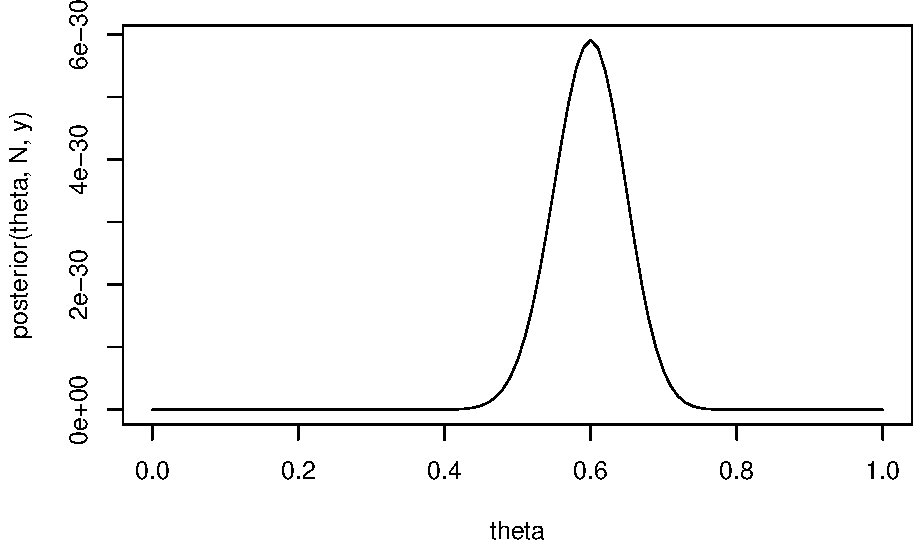
\includegraphics{BayesianDataAnalysisWorkbook_files/figure-latex/unnamed-chunk-1-1.pdf}

To interpret this, we have the unnormalized posterior density on the
Y-axis, and our only parameter, \(\theta\), on the X-axis. We see that
the probability of \(\theta\) being between out 0.5 and 0.7 is extremely
high. Well, we did have 60 successes out 100 trials, so it makes sense
that the underlying parameter for this would lie around 0.6.

One other key descriptive interval we can define for our posterior
distribution is the \textbf{highest posterior density region}, which is
the set of values that contains \(100(1-\alpha)\%\) of the posterior
probability. This is a useful interval similar to just a percentile
interval, but allows us to characterize distributions with e.g.~more
than one mode.

\section{Informative Priors}\label{informative-priors}

How do we go about constructing a prior though? There are two guides for
how to decide: first, under the population interpretation, the prior
distribution should represent a population of parameter values; second,
under the state of knowledge interpretation, the prior should represent
our knowledge (or uncertainty) about the parameter as if its value were
a random draw from the prior.

Typically, the prior should contain all possible realistic values of the
parameter, but need not be concentrated around any one value. Often, the
data will far outweigh the prior's information (NB: this makes me wonder
what the exact purpose of an intial prior is).

An alternative to the uniform prior distribution we used in our last
example is the Beta distribution. With the form
\(p(\theta)\propto \theta^{\alpha-1}(1-\theta)^{\beta-1}\), where we
have two parameters, \(\alpha\) and \(\beta\), which can be seen as
``prior successes'' and ``prior failures.'' These are also known as
\emph{hyperparameters}, as are any parameters of the prior distribution.

Applying Bayes' rule and we wind up with the posterior density for
\(\theta\) as:

\[
p(\theta|y) \propto \theta^y(1-\theta)^{n-y}\theta^{\alpha-1}(1-\theta)^{\beta-1} = \text{Beta}(\theta|\alpha+y, \beta+n-y)
\]

Which is to say, the binomial likelihood bound to a Beta prior leaves us
with a Beta posterior. When the posterior is of the same parametric form
as the prior, we call this a \emph{conjugate form}. Conjugate priors are
great because they're easy to compute (both analytically and
computationally), and they improve our ability to understand new data.

The standard distributions --- binomial, normal, Poisson, and
exponential --- have natural conjugate prior distributions, which can be
easily looked up. For an example though, we'll examine the Poisson
distribution and an example for it below.

\textbf{Poisson model}

The Poisson distribution appears when studying count data. The
probability distribution of a single observation is

\[
p(y|\theta) = \frac{\theta^ye^{-\theta}}{y!}\quad \text{for} y=0,1,2,\ldots
\]

Thus, if we have \(n\) IID observations, the likelihood is

\[
p(y|\theta) = \prod_{i=1}^n p(y_i|\theta) \propto \theta^{\sum_{i=1}^n y_i} e^{-n\theta}
\]

We'll skip some arithmetic found in the text and just say that the
conjugate prior for the Poisson distribution is

\[
p(\theta) \propto e^{-\beta\theta}\theta^{\alpha-1}
\]

which is a gamma density with parameters \(\alpha\) and \(\beta\):
Gamma(\(\alpha,\beta\)). With this prior, we can calculate the posterior
for the Poisson as

\[
\theta|y \sim \text{Gamma}(\alpha+n\bar{y},\beta + n)
\]

where \(n\) is the number of observed data and \(\bar{y}\) is the mean
of the IID observations.

\subsection{Estimating a rate from Poisson data: an idealized
example}\label{estimating-a-rate-from-poisson-data-an-idealized-example}

Suppose we're interested in modeling the number of people who die
annually due to asthma in a certain U.S. city. Let's say, last year we
know 3 out 200,000 people died, or roughly a mortality rate of 1.5 cases
per 100,000 persons per year.

We can express this via a sampling distribution of \(y\), the number of
deaths in a city of 200,000 in one year, as Poisson(\(2.0\theta\)),
where \(\theta\) represents the true underlying long-term asthma
mortality rate (measured in cases per 100,000 people per year). We have
our one observation, \(y=3\), and also the ``coefficient'' of 2.0, to
adjust for \(\theta\) being defined in terms of 100,000.

First, we'll establish a prior distribution. We can scour some previous
reports and find that in Western nations, the typical asthma mortality
rate is around 0.6 per 100,000 persons per year. We also believe that
it'll be very unlikely for rates to exceed 1.5 per 100,000. We know that
a convenient conjugate prior for the Poisson distribution is the gamma
distribution. Through a little trial and error, we find that
Gamma(\(3.0,5.0\)) gives a pretty good approximation to our world
knowledge: the mean is 0.6 and 97.5\% of the density is below 1.44.
Through a quick simulation we can verify this:
\texttt{mean(rgamma(1000,\ 3,\ 5))=0.601} and
\texttt{qgamma(0.975,\ 3,\ 5)=1.445}. This prior density takes the shape
of:

\begin{Shaded}
\begin{Highlighting}[]
\NormalTok{quantile =}\StringTok{ }\KeywordTok{seq}\NormalTok{(}\DecValTok{0}\NormalTok{,}\DecValTok{3}\NormalTok{,}\DataTypeTok{by=}\FloatTok{0.01}\NormalTok{)}
\KeywordTok{plot}\NormalTok{(quantile,}\KeywordTok{dgamma}\NormalTok{(quantile, }\DecValTok{3}\NormalTok{, }\DecValTok{5}\NormalTok{), }\DataTypeTok{type =} \StringTok{"l"}\NormalTok{)}
\end{Highlighting}
\end{Shaded}

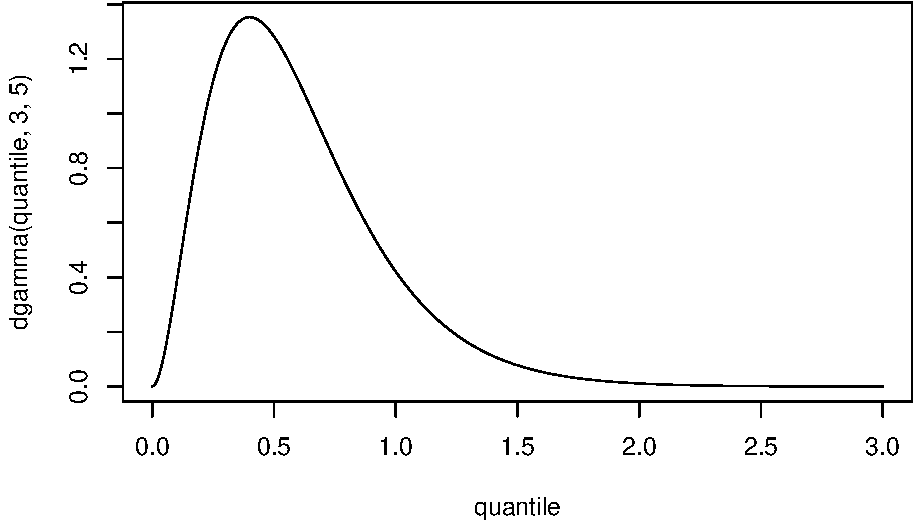
\includegraphics{BayesianDataAnalysisWorkbook_files/figure-latex/unnamed-chunk-2-1.pdf}

Given the likelihood and the prior, we can calculate the posterior
distribution, given above. With \(y=3.0\) and \(x=2\) (the
\emph{exposure} of the Poisson, described in the text), we can find the
new posterior parameters make

\[
\theta|y \sim \text{Gamma}(6.0, 7.0)
\]

Using this, for example, we can calculate the posterior probability that
the long-term mortality rate from asthma in this city being over,
e.g.~1.0 per 100,000 persons per year, is
\texttt{pgamma(1.0,\ 6,\ 7,\ lower.tail\ =\ F)=0.301}, or about 30.1\%.

There's a good exponential distribution example in the text that I won't
repeat here; I encourage it as review. One key topic I will mention
which is introduced in this example is the predicitive distribution ---
the marginal distribution of \(y\), averaging over the prior
distribution of \(\theta\) --- which is interpreted as the distribution
of possible unobserved values conditional on the observed ones.

\section{Noninformative and Weakly Informative
Priors}\label{noninformative-and-weakly-informative-priors}

Without knowledge of an underlying population, it can be difficult to
construct a prior distribution. Sometimes, one might instead construct a
vague, flat, diffuse, or \emph{noninformative} prior. Sometimes, one
might have a little knowledge of the population, and wish to construct a
\emph{weakly informative} prior. Noninformative priors can be
uncomfortably subjective (e.g.~if there is no clear choice for a vague
prior distribution) and introduce issues in later calculations of the
posterior. As the number of parameters in a given model grows, we may
wish to turn toward hierarchical models, something we'll get to later.

For an example, a noninformative prior on a binomial likelihood might be
the conjugates Beta(\(\frac{1}{2}, \frac{1}{2}\)) (the Jeffreys' prior
density based upon the Fisher Information of the binomial) or
Beta(\(1, 1\)) (the Bayes-Laplace uniform prior density). Yet, it is
still possibly to apply an uninformative prior if we go to the work to
check that the posterior density is finite for all \(y\) over
\(\int p(\theta|y)d\theta\) (it is \emph{proper}) and to check the
sensitivity of posterior inferences to our assumptions based upon
convenience (to be discussed).

We may, though, have some reasonably knowledge of the population
beforehand and wish to construct a \emph{weakly informative} prior. For
example, in a sex ratio problem, we may wish to begin modeling the
binomial data with Beta(\(20,20\)), which is centered at 0.5 and
contains a reasonable amount of information about the ratio of males to
females.

\section{Single-parameter Example}\label{single-parameter-example}

\begin{Shaded}
\begin{Highlighting}[]
\KeywordTok{library}\NormalTok{(tidyverse)}
\end{Highlighting}
\end{Shaded}

Suppose we have a Bulgarian friend named Georgi (Bulgarians don't get
enough recognition and Georgi is a good name). The average height of men
in Bulgaria is 5 ft 9 in. We don't however know the variance of this
estimate, so let's just say that most (95\%) of men are between 5 ft 5
in and 6 ft 1 in, thus the SD is \(\sigma = \frac{2}{12}\) (2 inches).
Now, Georgi just got his height measured for the first time in years.
What can we say about the national average then?

What's the probability, after adding Georgi's height to the national
database that the average Bulgarian man is taller than 6'? Our parameter
is the male Bulgarian height, and we have one data point (for Georgi),
and we have a value to compare to: 6 feet.

We use \(\mu\) to denote the height of Bulgarian men. We're pretending
that we know the population variance, \(\sigma^2 = \frac{1}{36}\). We
want to know, after adding Georgi's height \(y\), what is
P(\(\mu > 6 | \sigma^2, y\))?

We first need a likelihood and a prior. The likelihood \(p(y|\mu)\) is
the gaussian equation \(\mathcal{N}(y|\mu,\sigma^2)\). We'll choose a
conjugate prior for simplicity, another exponential of quadratic form
(just like the normal). This comes with two hyperparameters:
\(\mu \sim \mathcal{N}(\mu_0,\tau_0^2)\) (a mean and variance).

Here, \(\mu_0\) is our starting mean of \(5.75\) and we assume we know
our starting variance \(\tau_0^2 = \frac{1}{36}\). This is the same as
\(\sigma^2\) because our new sample of Georgi's height supposedly
follows this assumed variance. Let's set all our knowns right now:

\begin{Shaded}
\begin{Highlighting}[]
\NormalTok{parameter =}\StringTok{ }\KeywordTok{seq}\NormalTok{(}\FloatTok{4.5}\NormalTok{, }\DecValTok{7}\NormalTok{, }\DataTypeTok{by=}\FloatTok{0.01}\NormalTok{)}

\NormalTok{mu_}\DecValTok{0}\NormalTok{ =}\StringTok{ }\FloatTok{5.75} \CommentTok{# prior mean}
\NormalTok{sig_}\DecValTok{0}\NormalTok{ =}\StringTok{ }\DecValTok{1}\OperatorTok{/}\DecValTok{6} \CommentTok{# population SD}
\NormalTok{tau_}\DecValTok{0}\NormalTok{ =}\StringTok{ }\NormalTok{sig_}\DecValTok{0} \CommentTok{# prior SD}
\end{Highlighting}
\end{Shaded}

We can visualize our prior distribution over \(\mu\) given our starting
\(\mu_0\) and \(\tau_0^2\):

\begin{Shaded}
\begin{Highlighting}[]
\KeywordTok{plot}\NormalTok{(}\OtherTok{NA}\NormalTok{, }\DataTypeTok{xlim =} \KeywordTok{c}\NormalTok{(}\FloatTok{4.5}\NormalTok{, }\DecValTok{7}\NormalTok{), }\DataTypeTok{ylim =} \KeywordTok{c}\NormalTok{(}\DecValTok{0}\NormalTok{, }\DecValTok{1}\NormalTok{))}
\KeywordTok{lines}\NormalTok{(parameter, }\KeywordTok{exp}\NormalTok{(}\OperatorTok{-}\DecValTok{1}\OperatorTok{/}\NormalTok{(}\DecValTok{2}\OperatorTok{*}\NormalTok{tau_}\DecValTok{0}\OperatorTok{^}\DecValTok{2}\NormalTok{) }\OperatorTok{*}\StringTok{ }\NormalTok{(parameter }\OperatorTok{-}\StringTok{ }\NormalTok{mu_}\DecValTok{0}\NormalTok{)}\OperatorTok{^}\DecValTok{2}\NormalTok{), }\DataTypeTok{type =} \StringTok{"l"}\NormalTok{)}
\KeywordTok{abline}\NormalTok{(}\DataTypeTok{v =} \DecValTok{6}\NormalTok{)}
\end{Highlighting}
\end{Shaded}

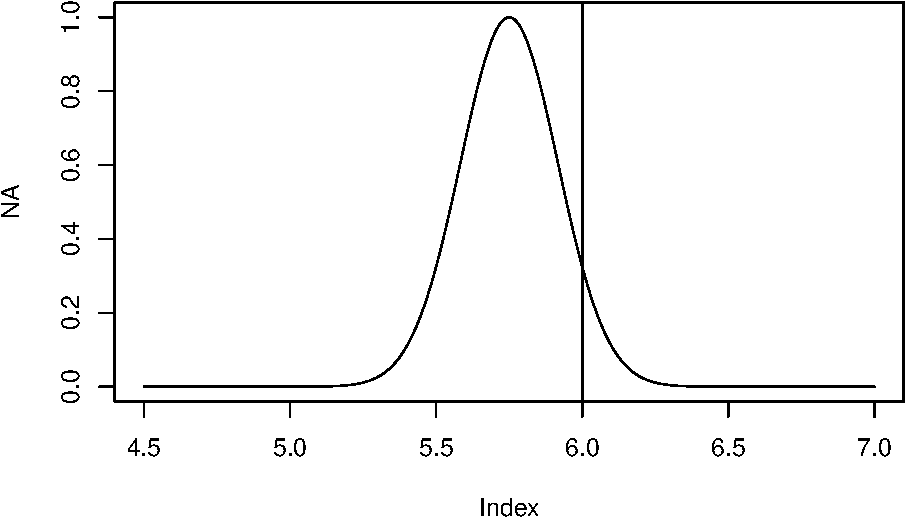
\includegraphics{BayesianDataAnalysisWorkbook_files/figure-latex/unnamed-chunk-5-1.pdf}

Only the x-axis are heights (4 ft 6 in to 7 ft 0 in) and on the y-axis
is the unnormalized density.

Using this, we can answer the question: without taking into any new
data, what's the probability that a man is taller than 6 ft?
\texttt{1-pnorm(6,\ mu\_0,\ tau\_0)} = 0.067 is the probability of
Bulgarian men, on our prior, being taller than 6 feet. Hence, there's
only a 6.7\% chance that a random sample from our prior of male
Bulgarian heights is over 6 ft!

The conjugate prior implies the posterior will take on the same form. We
can analytically determine the posterior by multiplying the prior and
the likelihood with the single datum:

\[
p(\mu|y) \propto \exp\big(-\frac{1}{2}\big(\frac{(y-\mu)^2}{\sigma^2} + \frac{(\mu - \mu_0)^2}{\tau_0^2}\big)\big)
\]

We can simplify this a bit for:

\[
p(\mu|y) \propto \exp\big(-\frac{1}{2\tau_1^2}(\mu - \mu_1)^2\big)
\]

where the terms were collected as:
\(\tau_1^2 = \frac{1}{1/\tau_0^2 + 1/\sigma_0^2}\) and
\(\mu_1 = \frac{\mu_0 / \tau_0^2 + y/\sigma^2}{1/\tau_0^2 + 1/\sigma^2}\).
This is all to say that we're incorporating our new datum into our known
information (the prior) by means of the likelihood. \(\tau_1^2\) and
\(\mu_1^2\) are updated parameters which we can use after this as well
with new data.

Translated into code:

\begin{Shaded}
\begin{Highlighting}[]
\NormalTok{posterior <-}\StringTok{ }\ControlFlowTok{function}\NormalTok{ (y) \{}
  \CommentTok{# set the posterior mean, a weighted average of the prior and the likelihood}
\NormalTok{  mu_}\DecValTok{1}\NormalTok{ <-}\StringTok{ }\NormalTok{(mu_}\DecValTok{0}\OperatorTok{/}\NormalTok{tau_}\DecValTok{0}\OperatorTok{^}\DecValTok{2} \OperatorTok{+}\StringTok{ }\NormalTok{y}\OperatorTok{/}\NormalTok{sig_}\DecValTok{0}\OperatorTok{^}\DecValTok{2}\NormalTok{) }\OperatorTok{/}\StringTok{ }\NormalTok{(}\DecValTok{1}\OperatorTok{/}\NormalTok{tau_}\DecValTok{0}\OperatorTok{^}\DecValTok{2} \OperatorTok{+}\StringTok{ }\DecValTok{1}\OperatorTok{/}\NormalTok{sig_}\DecValTok{0}\OperatorTok{^}\DecValTok{2}\NormalTok{)}
  
  \CommentTok{# set the posterior variance (note: not the SD, watch the exponentials later)}
\NormalTok{  tau_}\DecValTok{1}\NormalTok{ <-}\StringTok{ }\DecValTok{1}\OperatorTok{/}\NormalTok{(}\DecValTok{1}\OperatorTok{/}\NormalTok{tau_}\DecValTok{0}\OperatorTok{^}\DecValTok{2} \OperatorTok{+}\StringTok{ }\DecValTok{1}\OperatorTok{/}\NormalTok{sig_}\DecValTok{0}\OperatorTok{^}\DecValTok{2}\NormalTok{)}
  
  \KeywordTok{return}\NormalTok{(}\KeywordTok{list}\NormalTok{(}\DataTypeTok{mu_1 =}\NormalTok{ mu_}\DecValTok{1}\NormalTok{, }\DataTypeTok{tau_1 =}\NormalTok{ tau_}\DecValTok{1}\NormalTok{))}
\NormalTok{\}}
\end{Highlighting}
\end{Shaded}

Now, we measured Georgi at the beginning of this example. His height
ended up being 6 ft 5 in. He's a bit on the taller side, so how does
this change our belief about Bulgarian men being taller than 6 ft?

Here's the unnormalized prior and the unnormalized posterior (including
information about Georgi):

\begin{Shaded}
\begin{Highlighting}[]
\NormalTok{posterior_params <-}\StringTok{ }\KeywordTok{posterior}\NormalTok{(}\DecValTok{6} \OperatorTok{+}\StringTok{ }\DecValTok{5}\OperatorTok{/}\DecValTok{12}\NormalTok{) }\CommentTok{# 6 feet plus 5 inches}
\NormalTok{posterior_params}
\end{Highlighting}
\end{Shaded}

\begin{verbatim}
## $mu_1
## [1] 6.083333
## 
## $tau_1
## [1] 0.01388889
\end{verbatim}

\begin{Shaded}
\begin{Highlighting}[]
\CommentTok{# first, the prior in black}

\KeywordTok{plot}\NormalTok{(}\OtherTok{NA}\NormalTok{, }\DataTypeTok{xlim =} \KeywordTok{c}\NormalTok{(}\FloatTok{4.5}\NormalTok{,}\DecValTok{7}\NormalTok{), }\DataTypeTok{ylim =} \KeywordTok{c}\NormalTok{(}\DecValTok{0}\NormalTok{, }\FloatTok{1.1}\NormalTok{))}
\KeywordTok{lines}\NormalTok{(parameter, }\KeywordTok{exp}\NormalTok{(}\OperatorTok{-}\DecValTok{1}\OperatorTok{/}\NormalTok{(}\DecValTok{2}\OperatorTok{*}\NormalTok{tau_}\DecValTok{0}\OperatorTok{^}\DecValTok{2}\NormalTok{) }\OperatorTok{*}\StringTok{ }\NormalTok{(parameter }\OperatorTok{-}\StringTok{ }\NormalTok{mu_}\DecValTok{0}\NormalTok{)}\OperatorTok{^}\DecValTok{2}\NormalTok{), }\DataTypeTok{type =} \StringTok{"l"}\NormalTok{)}

\CommentTok{# second, the posterior in red (with a vertical line for 6 ft)}

\NormalTok{national_height <-}\StringTok{ }\DecValTok{6}
\KeywordTok{abline}\NormalTok{(}\DataTypeTok{v =}\NormalTok{ national_height)}

\KeywordTok{par}\NormalTok{(}\DataTypeTok{col =} \StringTok{"red"}\NormalTok{)}
\KeywordTok{lines}\NormalTok{(parameter, }\KeywordTok{exp}\NormalTok{(}\OperatorTok{-}\DecValTok{1}\OperatorTok{/}\NormalTok{(}\DecValTok{2}\OperatorTok{*}\NormalTok{posterior_params}\OperatorTok{$}\NormalTok{tau_}\DecValTok{1}\NormalTok{) }\OperatorTok{*}\StringTok{ }\NormalTok{(parameter }\OperatorTok{-}\StringTok{ }\NormalTok{posterior_params}\OperatorTok{$}\NormalTok{mu_}\DecValTok{1}\NormalTok{)}\OperatorTok{^}\DecValTok{2}\NormalTok{), }\DataTypeTok{type =} \StringTok{"l"}\NormalTok{)}
\end{Highlighting}
\end{Shaded}

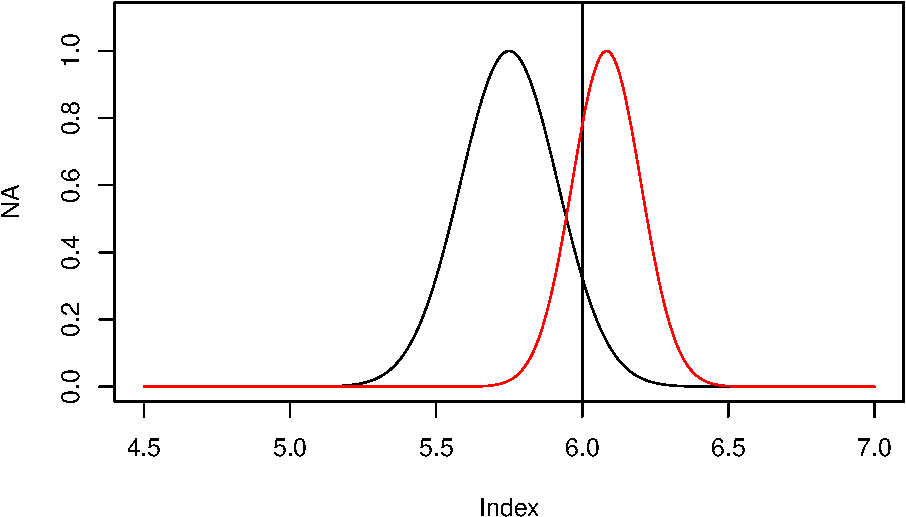
\includegraphics{BayesianDataAnalysisWorkbook_files/figure-latex/unnamed-chunk-7-1.pdf}

It's a little difficult to see, but the posterior density has gotten
slightly narrower to account for the increase in precision of the
estimate. We also see a pretty significant shift to the right.

What's the probability that a randomly sampled man in our posterior
distribution will be over 6 ft? By integration:
\texttt{1-pnorm(6,\ 6.0833,\ sqrt(0.01389))\ =\ 0.76}. We went from a
mere 7\% chance to now over 76\%! How?

\ldots{}

What's the probability that a randomly sampled \emph{future} man will be
over 6 ft given our one new measurement from Georgi? We will construct
the posterior predictive distribution, \(p(\tilde{y}|y)\), by
integrating out the parameter \(\mu\). Due to the uncertainty from the
start in \(\sigma^2\) and in \(\mu\) through \(\tau_1^2\), we add the
variances together to account for unknowns in the predictive variance:

\begin{Shaded}
\begin{Highlighting}[]
\DecValTok{1}\OperatorTok{-}\KeywordTok{pnorm}\NormalTok{(}\DecValTok{6}\NormalTok{, posterior_params}\OperatorTok{$}\NormalTok{mu_}\DecValTok{1}\NormalTok{, }\KeywordTok{sqrt}\NormalTok{(sig_}\DecValTok{0}\OperatorTok{^}\DecValTok{2} \OperatorTok{+}\StringTok{ }\NormalTok{posterior_params}\OperatorTok{$}\NormalTok{tau_}\DecValTok{1}\NormalTok{))}
\end{Highlighting}
\end{Shaded}

\begin{verbatim}
## [1] 0.6584543
\end{verbatim}

Or, approximately 66\% probability that a future man will be over 6 ft.

\chapter{Multi-Parameter Models}\label{multi}

Chapter 3 - To be completed

\begin{Shaded}
\begin{Highlighting}[]
\NormalTok{dnorminchi <-}\StringTok{ }\ControlFlowTok{function}\NormalTok{ (mu, sig, mu_}\DecValTok{0}\NormalTok{, k_}\DecValTok{0}\NormalTok{, sig_}\DecValTok{0}\NormalTok{, v_}\DecValTok{0}\NormalTok{, y) \{}
\NormalTok{  y_mean <-}\StringTok{ }\KeywordTok{mean}\NormalTok{(y)}
\NormalTok{  n <-}\StringTok{ }\KeywordTok{length}\NormalTok{(y)}
  
\NormalTok{  mu_n <-}\StringTok{ }\NormalTok{(k_}\DecValTok{0} \OperatorTok{*}\StringTok{ }\NormalTok{mu_}\DecValTok{0}\NormalTok{)}\OperatorTok{/}\NormalTok{(k_}\DecValTok{0} \OperatorTok{+}\StringTok{ }\NormalTok{n) }\OperatorTok{+}\StringTok{ }\KeywordTok{sum}\NormalTok{(y)}\OperatorTok{/}\NormalTok{(k_}\DecValTok{0} \OperatorTok{+}\StringTok{ }\NormalTok{n)}
\NormalTok{  k_n <-}\StringTok{ }\NormalTok{k_}\DecValTok{0} \OperatorTok{+}\StringTok{ }\NormalTok{n}
\NormalTok{  sig_n <-}\StringTok{ }\NormalTok{sig_}\DecValTok{0}
\NormalTok{  v_n <-}\StringTok{ }\NormalTok{v_}\DecValTok{0} \OperatorTok{+}\StringTok{ }\NormalTok{n}
  
  \KeywordTok{return}\NormalTok{(sig}\OperatorTok{^-}\DecValTok{1} \OperatorTok{*}\StringTok{ }\NormalTok{(sig}\OperatorTok{^}\DecValTok{2}\NormalTok{)}\OperatorTok{^}\NormalTok{(}\OperatorTok{-}\NormalTok{(v_n}\OperatorTok{/}\DecValTok{2} \OperatorTok{+}\StringTok{ }\DecValTok{1}\NormalTok{)) }\OperatorTok{*}\StringTok{ }
\StringTok{           }\KeywordTok{exp}\NormalTok{((mu}\OperatorTok{-}\NormalTok{mu_n)}\OperatorTok{^}\DecValTok{2}\NormalTok{))}
\NormalTok{\}}

\NormalTok{dmarginal_mu <-}\StringTok{ }\ControlFlowTok{function}\NormalTok{ (mu, mu_}\DecValTok{0}\NormalTok{, sig_}\DecValTok{0}\NormalTok{, k_}\DecValTok{0}\NormalTok{, v_}\DecValTok{0}\NormalTok{, y) \{}
  
\NormalTok{  y_mean <-}\StringTok{ }\KeywordTok{mean}\NormalTok{(y)}
\NormalTok{  n <-}\StringTok{ }\KeywordTok{length}\NormalTok{(y)}
  
\NormalTok{  mu_n <-}\StringTok{ }\NormalTok{(k_}\DecValTok{0} \OperatorTok{*}\StringTok{ }\NormalTok{mu_}\DecValTok{0}\NormalTok{)}\OperatorTok{/}\NormalTok{(k_}\DecValTok{0} \OperatorTok{+}\StringTok{ }\NormalTok{n) }\OperatorTok{+}\StringTok{ }\KeywordTok{sum}\NormalTok{(y)}\OperatorTok{/}\NormalTok{(k_}\DecValTok{0} \OperatorTok{+}\StringTok{ }\NormalTok{n)}
\NormalTok{  k_n <-}\StringTok{ }\NormalTok{k_}\DecValTok{0} \OperatorTok{+}\StringTok{ }\NormalTok{n}
\NormalTok{  v_n <-}\StringTok{ }\NormalTok{v_}\DecValTok{0} \OperatorTok{+}\StringTok{ }\NormalTok{n}
\NormalTok{  sig_n <-}\StringTok{ }\NormalTok{v_}\DecValTok{0} \OperatorTok{*}\StringTok{ }\NormalTok{sig_}\DecValTok{0}\OperatorTok{^}\DecValTok{2} \OperatorTok{+}\StringTok{ }\NormalTok{(n}\OperatorTok{-}\DecValTok{1}\NormalTok{)}\OperatorTok{*}\KeywordTok{var}\NormalTok{(y) }\OperatorTok{+}\StringTok{ }\NormalTok{k_}\DecValTok{0} \OperatorTok{*}\StringTok{ }\NormalTok{n }\OperatorTok{*}\StringTok{ }\NormalTok{(y_mean }\OperatorTok{-}\StringTok{ }\NormalTok{mu_}\DecValTok{0}\NormalTok{)}\OperatorTok{^}\DecValTok{2} \OperatorTok{/}\StringTok{ }\NormalTok{(k_}\DecValTok{0} \OperatorTok{+}\StringTok{ }\NormalTok{n)}
\NormalTok{  sig_n <-}\StringTok{ }\NormalTok{sig_n }\OperatorTok{/}\StringTok{ }\NormalTok{v_n}
  
  \KeywordTok{print}\NormalTok{(}\KeywordTok{c}\NormalTok{(mu_n, k_n, sig_n, v_n))}
  
  \KeywordTok{return}\NormalTok{(}\KeywordTok{list}\NormalTok{(}\DataTypeTok{mu =}\NormalTok{ (mu }\OperatorTok{-}\StringTok{ }\NormalTok{mu_n)}\OperatorTok{^}\DecValTok{2} \OperatorTok{*}\StringTok{ }\NormalTok{k_n }\OperatorTok{/}\StringTok{ }\NormalTok{sig_n}\OperatorTok{^}\DecValTok{2}\NormalTok{, }\DataTypeTok{df =}\NormalTok{ v_n,}
           \DataTypeTok{mu_n =}\NormalTok{ mu_n, }\DataTypeTok{k_n =}\NormalTok{ k_n, }\DataTypeTok{sig_n =}\NormalTok{ sig_n, }\DataTypeTok{v_n =}\NormalTok{ v_n))}
\NormalTok{\}}
\end{Highlighting}
\end{Shaded}

\begin{Shaded}
\begin{Highlighting}[]
\CommentTok{# mu <- seq(-10, 10, by=0.1)}
\CommentTok{# plot(NA, xlim = c(-10, 10), ylim = c(0, 0.5))}
\CommentTok{# posterior <- dmarginal_mu(mu, 1, 10, 0, 0, c(1,2))}
\CommentTok{# lines(mu, dt(posterior$mu, posterior$df))}
\CommentTok{# }
\CommentTok{# par(col = "red")}
\CommentTok{# lines(mu, dmarginal_mu(mu, posterior$mu_n, posterior$sig_n, posterior$k_n, posterior$v_n, }
\CommentTok{#                        c(-4,-7,-8,-5,-4,3,2)))}
\CommentTok{# }
\CommentTok{# par(col = "orange")}
\CommentTok{# lines(mu, dmarginal_mu(mu, 1, 10, 0, 0, c(-4,-7,-8,-5,-4,3,2,2,2,2,2,2,2)))}
\CommentTok{# }
\CommentTok{# par(col = "yellow")}
\CommentTok{# lines(mu, dmarginal_mu(mu, 1, 10, 0, 0, c(-4,-7,-8,-5,-4,3,2,2,2,2,2,2,2,3,3,3,3,3,3,3)))}
\end{Highlighting}
\end{Shaded}

\bibliography{book.bib,packages.bib}

\end{document}
